\documentclass[../main.tex]{subfiles}

\begin{document}

\chapter{Data and Data Processing}
\label{chap:data}
This will be a summary of the data we use in this project and some data which we don't (but is used by other researchers)
How is it collected? What format is it in?
How reliable is it?
This chapter will also contain a brief overview of some of the preprocessing methods carried out on the variety of datasets used for this project. 



\section{Antarctic Ice}
\subsection*{Sea Ice}

\subsection*{Thickness of sea ice}
For this project we are also interest in using the thickness of Antarctic Sea Ice to aid our analyses. This is complicated because measuring the thickness of ice in Antarctica involves a number of technical challenges. Satellites have been used since the late 90s for measuring ice concentration, as described above this involves measuring the albedo of regions with ice and using the measured values as a proxy for the amount of ice. A number of satellite missions have been used to carry this out. We cannot use the same data as for land ice thickness (described below) because that data includes all liquid water in its thickness calculations as well as frozen ice. So we have to turn to other sources of data. These sources are varied, and none of great quality for Antarctica, so we will pick one which seems to give us reasonable values and use it for qualitative rather than quantitative understanding of the behaviour of ice in Antarctica.

One we settled on is collected by NASA's Ice, Cloud, and land Elevation Satellite (ICEsat). This data has been processed by Kurtz and Markus \textcolor{red}{cite}. It is freely available online (insert website here)[]. Limitations we have to consider are that the time period for the data is limited to between 2003-2008. As such we cannot reliably use it for extended periods of time but will use it briefly in our research. Additionally they only have data for Spring, Summer and Autumn, not winter, so we are missing the time of year with the thickest amount of ice.  For use in this project, we will treat this data as a rough indicator for how thick ice can be around Antarctica and treat any calculations using it as rough estimates which can be used to indicate potential relationships but require better data.

The data is in our standard polar stereographic projection of 25km x 25km, \textcolor{red}{link this here} so no interpolation is necessary. In order to obtain an approximate thickness of ice on an annual scale, we will average these three datasets together and use this as our value for the thickness of ice. Because the data is limited in nature this is for qualitative understanding only.

\subsection*{Land Ice}
\subsection*{Standardising Ice values}

We can try to standardise the different ice datasets so we can use them as one variable without comparing them separately.

The NSIDC data comes in a concentration \% with an associated area data file. We can therefore calculate the total area of ice which changes from year to year, or leave the data as a \%.

The GRACE data



\section{Environmental variables}

\subsection{Describing the environmental variables}

For this project we use ERA5 reanalysis data produced by ECMWF \textcolor{red}{cite this} as our source of data for the environmental variables listed below.

\begin{itemize}
	\item Skin Temperature [SKT]
	\item 2 metre Temperature [T2M]
	\item Sea Surface Temperature [SST]
\end{itemize}

This data comes in a regular \textcolor{red}{check resolution} 0.25 degrees grid which covers the entire globe. For our analysis which involves looking at weather in Antarctica we projected this data onto the standard South Polar Stereographic projection as defined by NSIDC \textcolor{red}{link this here}.
This means that the data we use for analysis is interpolated which lowers the quality slightly, but negligibly in compared to the utility we gain from having it in the same projection and coordinates as our other sources of data.
Next we should consider the different variables we used from this dataset. Listed above, we will now go through them one by one and explain how they are calculated and what this may mean for the project and any results we may generate.
For a full technical description of how any and all variables are calculated for the ERA5 reanalysis you can refer to \textcolor{red}{cite report}. We will briefly summarise the most relevant points here for convenience of the reader.

\subsubsection*{Skin Temperature [SKT]}

The skin temperature is the theoretical temperature that is required to satisfy the surface energy balance. It represents the temperature of the uppermost surface layer, which has no heat capacity and so can respond instantaneously to changes in surface fluxes. Skin temperature is calculated differently over land and sea because of the difference in dynamics in each type of terrain.

In the presence of sea ice, skin temperature is taken as the temperature on the upper surface of the ice.

\subsubsection*{2 metre Temperature [T2M]}

2 metre temperature is the temperature measurement which is most often used in literature because of its regularity. 2m temperature is calculated by interpolating between the lowest model level \textcolor{red}{check what pressure this is} and the Earth's surface, taking account of the atmospheric conditions.

\subsubsection*{Sea Surface Temperature [SST]}

SST is usually calculated directly from satellite data, but in the absence of that it is calculated using data from NEMO forecasts 
\textcolor{red}{cite this}.
Sea surface temperature is masked to be only over sea and as such we can only use it when doing calculations over the ocean. Nonetheless it is still useful.
When the ocean is exposed this will be very similar to skin temperature, however when sea ice is found, SST is usually set to -1.65$^\circ$C, the freezing point for salt water. 

\subsection{Example plots}


\subsection{Validation}
We can validate the quality of our temperature data sourced from the ERA5 reanalysis by comparing the reanalyssis with measured station temperature data. This is included below
\begin{figure}[h!]
    \centering
    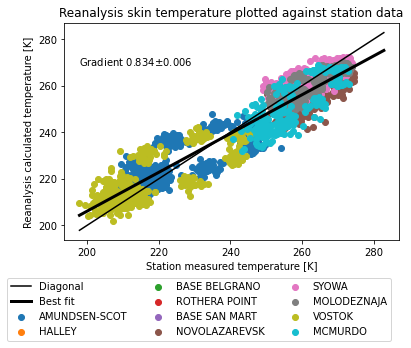
\includegraphics{images/week7/lres/temperature_station_verification_scatter}
    \caption{Reanalysis and measured temperature scatter plot.}
    \label{fig:temperature_station_verification_scatter}
\end{figure}



\section{Climate Indices}
\subsection*{SAM}
\subsection*{ENSO}
\subsection*{DMI}
\subsection*{IPO}
\subsection*{Non-Pacific Climate Modes}


\section{Pre-processing}
\subsection*{Temporal Averaging}
\subsection*{Spatial Regridding}
Because we use a variety of datasets which come in a variety of structures, it is important that standardise the spatial dimensions of each data source. One way we do this is by interpolating each dataset to have a consistent spatial arrangement. This allows for better quality results and makes it easier to calculate measures such as the correlation between 2m temperature and sea ice concentration.

We do the interpolation using the python package Scipy, which makes use of a piece-wise cubic, continuously differentiable (C1), and approximately curvature-minimising polynomial surface to determine the value of our given variable at a chosen location. 

We converted the temperature data to the projection the sea ice data is provided in; a south polar stereographic projection with regular grid cells of 25km$\times$25km. We found this resolution to have a good balance between reasonable run-times and good quality results.

\subsection*{Temporal Anomalies}
\subsection*{Erroneous Values}

\end{document}